\documentclass[12pt]{article}
\usepackage{graphicx}
\usepackage[utf8]{inputenc}
\usepackage[english]{babel}
\usepackage{fullpage}
\usepackage{listings}
\usepackage{xcolor}
\usepackage{url}
\usepackage[linesnumbered,ruled,vlined]{algorithm2e}
\usepackage{enumitem}
\usepackage{mathrsfs}
\usepackage{amssymb}
\usepackage{amsmath}
\usepackage{enumitem}
\usepackage{hyperref}
\usepackage{float}
\usepackage{sbc-template}


\definecolor{mygreen}{rgb}{0,0.6,0}

\hypersetup{
    colorlinks=true,
    linkcolor=cyan,
    urlcolor=cyan}

\newcounter{problem}
\newcounter{solution}

\pagestyle{plain}
\thispagestyle{plain}

\newtheorem{prop}{Proposição}
\newtheorem{ex}{Exemplo}[section]
\newtheorem{theorem}{Teorema}
\newtheorem{corollary}{Corolário}[theorem]
\newtheorem{lemma}[theorem]{Lemma}
\newtheorem{definition}{Definição}

\lstset{ % lstlisting
    language=Python,
    frame=tb, % draw a frame at the top and bottom of the code block
    tabsize=4, % tab space width
    showstringspaces=false, % don't mark spaces in strings
    commentstyle=\color{mygreen}, % comment color
    keywordstyle=\color{blue}, % keyword color
    stringstyle=\color{red}, % string color
    numbers=left, 
    numbersep=9pt,
    backgroundcolor=\color{black!5}, % set backgroundcolor
    basicstyle=\footnotesize,% basic font setting
}

\newcommand{\furl}[1]{\footnote{\url{#1}}}

\newcommand\Problem{%
  \stepcounter{problem}%
  \textbf{Problema \theproblem:}
  \setcounter{solution}{0}%
}

\newcommand\TheSolution{%
  \textbf{Solução:}\\%
}

\newcommand\ASolution{%
  \stepcounter{solution}%
  \textbf{Solução \thesolution:}\\%
}
% \parindent0in
\parskip 1.5em

\title{Curso de Curvas e Superfícies}

\author{Wellington José Leite da Silva\inst{1}}

\address{Escola de Matemática Aplicada da FGV (EMAP), Brazil}

\date{}

\begin{document}

\maketitle

%\section*{Sumário}

%\textbf{\nameref{s1}}

%\textbf{\nameref{s2}}
%\vspace{4.0mm}

%\textbf{\nameref{s3}}
%\vspace{4.0mm}


\section*{Apresentação}\label{s1}
Apresentamos aqui uma linha de aprendizado do curso de curvas e superfícies apresentando definições, teoremas e etc. Com intuído de auxiliar o aprendizado aos tópicos apresentados no mesmo e fornecer uma forma de visualização computacional a partir dos exemplos usando \textit{sagemath}. Aqui seguimos principalmente o livro \cite{bookmain} e adicionando sempre que possível, exemplos ilustrativos usando o \textit{sagemath}. As implementações, códigos usados para as mesmas assim como o \textit{Tex} deste documento se concentram no repositório curvas-superficies no github \furl{https://github.com/wellington36/curvas-superficies}.

\section{Curvas regulares}\label{s2}

\begin{definition}
Uma \textbf{curva parametrizada} $\alpha$ em $\mathbb{R}^n$ é uma aplicação $\gamma: I \rightarrow \mathbb{R}^n$ sendo $I \subset \mathbb{R}$ aberto, da forma

$$\alpha(t) = (x(t), y(t)),\ t\in I$$

onde x e y são funções diferenciáveis de t.
\end{definition}

\begin{ex}[Curva parametrizada diferenciável] A curva 

$$\alpha(t) = (1/2 \cos(t) + 1/3 \sin(4 t), 1/2 \sin(t) + 1/3 \cos(4 t))$$ 

é um exemplo de curva parametrizada diferenciável e podemos visualizar no \textit{sagemath} da seguinte forma
\begin{lstlisting}
# curve definition
curve_alpha(t) = (1/2 * cos(t) + 1/3 * sin(4 * t), 
                  1/2 * sin(t) + 1/3 * cos(4 * t))

# plot
parametric_plot(curve_alpha, (t,0, 2*pi), thickness=2)
\end{lstlisting}

\begin{figure}[H]
    \centering
    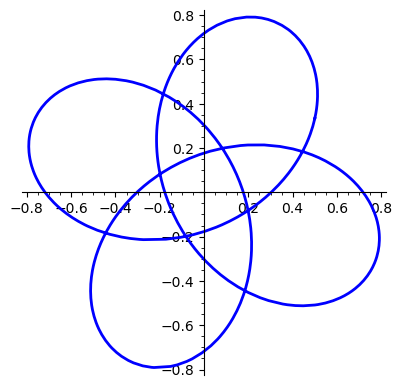
\includegraphics[scale=.6]{Images/ex1.1.png}
    \caption{Curva parametrizada}
    \label{fig:ex1.1}
\end{figure}
\end{ex}

\begin{definition}
O conjunto imagem de uma curva $\gamma$, $\gamma(I) \subset \mathbb{R}^n$ é dito o \textbf{traço} de $\gamma$.
\end{definition}

\begin{definition}[Vetor tangente]
Seja $\gamma: I \rightarrow \mathbb{R}^n$ com $\gamma(t) = (\gamma_1 (t), \ldots, \gamma_n (t))$ com $\gamma_i (y)$ diferenciáveis $\forall i, i = 1 \ldots n$, o vetor

$$\gamma'(t) = (\gamma'_1 (t), \ldots, \gamma'_n (t))$$

é chamado \textbf{vetor tangente de $\gamma$} em t
\end{definition}

\begin{ex}[Vetores tangentes] Usando a mesma curva acima podemos visualizar os vetores tangentes da seguinte forma
\begin{lstlisting}
M = Manifold(2, 'M')
X.<x,y> = M.chart()

c = M.curve([1/2 * cos(t) + 1/3 * sin(4 * t), 
             1/2 * sin(t) + 1/3 * cos(4 * t)], (t, 0, 2*pi))

v = c.tangent_vector_field() ; v

show(c.plot(thickness=2, aspect_ratio=1) +
     v.plot(chart=X, number_values=30, scale=.2))
\end{lstlisting}

\begin{figure}[H]
    \centering
    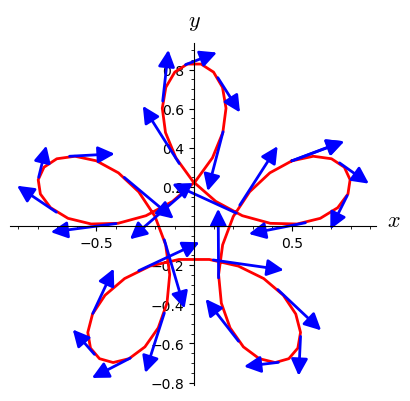
\includegraphics[scale=.6]{Images/ex1.2.png}
    \caption{Vetores tangentes}
    \label{fig:ex1.2}
\end{figure}

\end{ex}

\begin{definition}[Curvas regulares]
Seja $\gamma (t): I \rightarrow \mathbb{R}^n$ uma curva parametrizada diferenciável. Diz-se que \textbf{$\gamma$ é regular}, quando $\gamma'(t) \neq 0,\ \forall t \in I$.
\end{definition}

\begin{definition}[Comprimento de arco]
O \textbf{comprimento de arco de $\alpha$}, de $\alpha(a)$ até $\alpha(b)$ definido por $L_a^b (\alpha)$ é  

$$L_a^b (\alpha) = \int_a^b \| \alpha'(t) \| d t$$
\end{definition}

\begin{ex}[Comprimento de arco] O comprimento de arco da curva $\alpha(t) = (2 \cos(t), 2 \sin(t))$ pode ser encontrada fazendo
\begin{lstlisting}
curve_alpha(s) = (2 * cos(s), 2 * sin(s))

x = get_vector_arguments(curve_alpha).pop()
curve_alpha_x = curve_alpha.derivative(x)
    
# Calcular comprimento de arco de 0 a t
t = var("t")
assume(t>0)
s = integrate(norm(curve_alpha_x), (x,0,t))
s = s.simplify_full()

pretty_results((r"\int_0^t || C'(x) || dx", s))
\end{lstlisting}

\newcommand{\Bold}[1]{\mathbf{#1}}\begin{align*} \int_0^t || C'(x) || dx &= 2t \\ \end{align*}
\end{ex}

\begin{definition}
Se $\gamma: (a, b) \rightarrow \mathbb{R}^n$ é uma c.p.\footnote{curva parametrizada}, sua \textbf{velocidade no ponto} $\gamma(t)$ é $\| \gamma'(t) \|$, e a curva é dita com \textbf{velocidade unitária} se $\| \gamma'(t) \| = 1,\ \forall t \in (a, b)$ e é parametrizada por comprimento de arco.
\end{definition}

\begin{theorem}
Toda \textbf{curva regular} pode ser reparametrizada por \textbf{comprimento de arco}.
\end{theorem}


\section{Difeomorfismo e Reparametrizacao}\label{s3}
\begin{definition}[Difeomorfismo]
Dado os conjuntos abertos $U \subset \mathbb{R}^n$ e $V \subset \mathbb{R}^n$. Uma bijeção $f: U \rightarrow V$ é dita \textbf{difeomorfismo} quando f e $f^{-1}$ são diferenciáveis.
\end{definition}

\begin{definition}[Reparametrização]
A curva $\beta(s)$ é dita uma \textbf{reparametrização} de $\alpha(t): I \subset \mathbb{R} \rightarrow \mathbb{R}^2$ regular quando dados $I_0 \subset \mathbb{R}$ e $\phi: I_0 \rightarrow I$ difeomorfismo. Temos $\beta(S) = \alpha(\phi(S)))$.
\end{definition}

\begin{definition}
Seja $\alpha(t): (a, b) \rightarrow \mathbb{R}^2$ r $\beta(S): (c, d) \rightarrow \mathbb{R}^2$. Então

\begin{itemize}
    \item $\beta(S)$ é uma reparametrização positiva de $\alpha$ se $\phi'(S) > 0,\ \forall S$
    \item $\beta(S)$ é uma reparametrização negativa de $\alpha$ se $\phi'(S) < 0,\ \forall S$
\end{itemize}
\end{definition}

\begin{definition}
Qualquer reparametrização de uma c.p. regular é regular (i.e. difeomorfismos preservam regularidade).
\end{definition}

\begin{ex}[Reparametrização por difeomorfismo]
Seja a seguinte curva (que vou chamar aqui de flor)

$$\alpha(t) = (\cos(t) + \sin(4 t), \sin(t) + \cos(4 t))$$

podemos reparametrizar digamos pela função $\phi(t) = 2 t + 1$ da seguinte forma, como de costume usando \textit{sagemath}

\begin{lstlisting}
# curve definition
alpha(t) = (cos(t) + sin(4 * t), sin(t) + cos(4 * t))

# reparametrization
phi(x) = 2 * x + 1
beta(t) = alpha(phi(t))

# plot
parametric_plot(alpha, (t,0, 2*pi), thickness=2)
parametric_plot(beta, (t,0, 2*pi), thickness=2, color='red')
\end{lstlisting}

\begin{figure}[H]
    \centering
    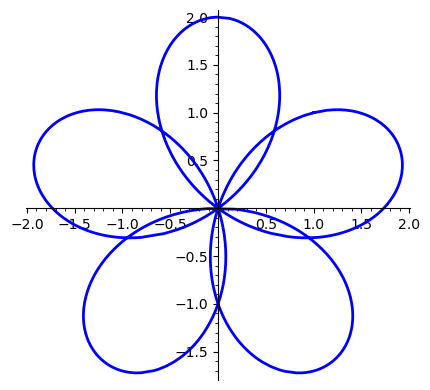
\includegraphics[scale=.6]{Images/ex2.1-1.png}
    \caption{Curva $\alpha$}
    \label{fig:ex2.1-1}
\end{figure}

\begin{figure}[H]
    \centering
    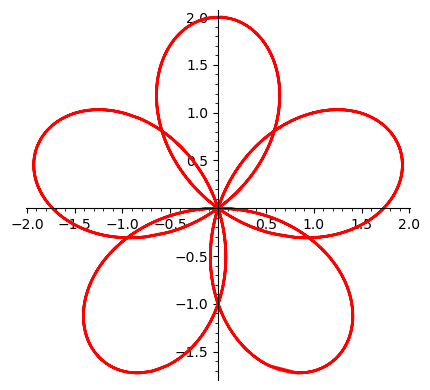
\includegraphics[scale=.6]{Images/ex2.1-2.png}
    \caption{Curva $\alpha$ reparametrizada}
    \label{fig:ex2.1-2}
\end{figure}

Aqui $\phi$ é um difeomorfismo gerando uma reparametrização de $\alpha$ em particular o traço das curvas se mantém e $\beta$ é uma reparametrização positiva
\end{ex}

\begin{prop}
A função L (comprimento de arco) é um difeomorfismo.
\end{prop}

\begin{definition}
Toda curva regular $\alpha: I \rightarrow \mathbb{R}^2$ admite reparametrização por comprimento de arco.
\end{definition}

\begin{ex}[Reparametrização por comprimento de arco]
Usaremos aqui a mesma curva usada para calcular o comprimento de arco no caso o círculo de raio 2 $\alpha(t) = (2 \cos(t), 2 \sin(t))$, com ela podemos obter sua parametrização por comprimento de arco fazendo os seguintes passos

\begin{lstlisting}
# curve definition
alpha(s) = (2 * cos(s), 2 * sin(s))

# Identify curve parameter
x = get_vector_arguments(alpha).pop()

# Calculate the derivatives
curva_x = alpha.derivative(x)
    
# Calculate arc length from 0 to t
t = var("t")
assume(t>0)
comp_arco = integrate(norm(curva_x), (x,0,t))

t = comp_arco.arguments()[0]
    
# Find t in terms of s
s = var("s")
param_comp_arco = solve(s == comp_arco,t)[0]
    
# Replace original parameter in curve 
curva_subs = alpha(t).subs(param_comp_arco)
curva_subs = vector_simplify(curva_subs)
    
# Reset function argument
curva_param(s) = tuple(coord for coord in curva_subs)

# New curve plot
pretty_results((r"C(s)", curva_param), use_colon=True)
\end{lstlisting}

\newcommand{\Bold}[1]{\mathbf{#1}}\begin{align*} C(s) :& \quad s \ {\mapsto}\ \left(2 \, \cos\left(\frac{1}{2} \, s\right),\,2 \, \sin\left(\frac{1}{2} \, s\right)\right) \\ \end{align*}

A mesma sequência de comandos pode ser facilmente reproduzida em outras curvas. 
\end{ex}

\section{Curvatura}\label{s4}

\begin{definition}[Função Ângulo]
Dada uma curva diferenciável $\gamma: I \rightarrow S^1$, onde $S^1$ é o círculo de $\mathbb{R}^2$ com centro na origem e raio 1, diz-se que $\theta: I \rightarrow \mathbb{R}$ é uma \textbf{função-ângulo} de $\gamma$, quando

$$\gamma(s) = (\cos(\theta(s)), \sin(\theta(s)),\ \forall s \in I$$
\end{definition}

\begin{definition}[Curvatura]
Seja $\alpha: I \rightarrow \mathbb{R}$ unit-speed. Designando-se o vetor tangente de $\alpha$ em $s \in I$ por $T(s)$, podemos afirmar que a curva $T(s) = I \rightarrow S^1$ admite função ângulo

$$T(s) = (\cos(\theta(s)), \sin(\theta(s)),\ \forall s \in I$$

Daí a \textbf{curvatura} de $\alpha$ em $s \in I$ é definida por

$$K(s) = \theta'(s) = det(\alpha'(s), \alpha''(s))$$
\end{definition}

\begin{ex}[Exemplo curvatura] A curvatura da curva $\alpha(t) = (2\sin(t), 2\cos(t))$, pode ser calculada fazendo
\begin{lstlisting}
# define the curve
curve(t) = (2 * cos(t), 2 * sin(t))

# calculate the derivatives
curve_t = curve.derivative(t)
curve_tt = curve_t.derivative(t)

# calculate J(c'(t))
curve_t_rotation(t) = (- curve_t[1], curve_t[0])

# calculate the curvature
curvatura = curve_t_rotation.dot_product(curve_tt)/norm(curve_t)^3
curvatura = curvatura.simplify_full()

# plot
pretty_results((r"K(s)", curvatura), use_colon=True)
\end{lstlisting}

\newcommand{\Bold}[1]{\mathbf{#1}}\begin{align*} K(s) :& \quad \frac{1}{2} \\ \end{align*} \\

Em geral, a curvatura de $\alpha(t) = (r \sin(t), r \cos(t)),\ \forall r \in \mathbb{R} - \{0\}$ é $K_\alpha(t) = \frac{1}{r}$
\end{ex}

\section{Diedro de Frenet e Teorema Fundamental}\label{s4}
\begin{theorem}[Função-ângulo diferenciável]
Seja $\gamma: I \rightarrow S^1$ uma curva diferenciável. Então, $\gamma$ admite uma função ângulo $\theta: I \rightarrow \mathbb{R}$, a qual é diferenciável. Além disso, toda função-ângulo de $\gamma$, a qual é diferenciável, difere de $\theta$ por uma constante.
\end{theorem}

\begin{corollary}
Seja $\alpha : I \subset \mathbb{R} \rightarrow \mathbb{R}$ e seja $\beta(s) = \alpha(\theta(s))$ a parametrização por comprimento de arco de $\alpha$, a curvatura de $\alpha$ em $t \in I$ é $K_\alpha(t)$, e, por definição é a curvatura de $\beta$ em $\theta^{-1}(t)$, isto é

$$K_\alpha := K_\beta(\theta^{-1}(t))$$
\end{corollary}

\begin{definition}[Diedro de Frenet]
Seja $\alpha: I \subset \mathbb{R} \rightarrow \mathbb{R}^2$ uma curva regular parametrizada por comprimento de arco. Dado $s \in I$, o vetor $N(s) = JT(s)$ é dito o vetor normal de $\alpha$ em $s \in I$. A base ortonormal de $\mathbb{R}^2$ formado por $T(s)$ e $N(s)$ é chamada \textbf{Dietro de Frenet} em s.
\end{definition}

\begin{ex}[Diedro de Frenet] Vamos encontrar aqui os vetores T e N do Diedro de Frenet da curva $\alpha(t) = (\sin(2 t), \cos(t))$

\begin{lstlisting}
# Curve definition
alpha(t) = (sin(2 * t), cos(t))

# Diedro de Frenet
T(t) = alpha.derivative(t)/norm(alpha.derivative(t))

N(t) = (- T[1], T[0])

# Plot
pretty_results((r"T(t)", T))
pretty_results((r"N(t)", N))
\end{lstlisting}

\newcommand{\Bold}[1]{\mathbf{#1}}\begin{align*} T(t) :& \quad t \ {\mapsto}\ \left(\frac{2 \, \cos\left(2 \, t\right)}{\sqrt{4 \, \cos\left(2 \, t\right)^{2} + \sin\left(t\right)^{2}}},\,-\frac{\sin\left(t\right)}{\sqrt{4 \, \cos\left(2 \, t\right)^{2} + \sin\left(t\right)^{2}}}\right) \\ \end{align*}

\begin{align*} N(t) :& \quad t \ {\mapsto}\ \left(\frac{\sin\left(t\right)}{\sqrt{4 \, \cos\left(2 \, t\right)^{2} + \sin\left(t\right)^{2}}},\,\frac{2 \, \cos\left(2 \, t\right)}{\sqrt{4 \, \cos\left(2 \, t\right)^{2} + \sin\left(t\right)^{2}}}\right) \\ \end{align*} \\
\end{ex}

\begin{definition}[Movimento Rígido]
$\Phi: \mathbb{R}^2 \rightarrow \mathbb{R}^2$ é dita \textbf{movimento rígido}, quando preserva distancia, isto é, para quaisquer $p, q \in \mathbb{R}^2$

$$\| \Phi(p) - \Phi(q) \| = \| p - q \|$$
\end{definition}

\begin{theorem}
Seja $\Phi: A + p_0$ um movimento rígido direto de $\mathbb{R}^2$ e $\alpha: I \rightarrow \mathbb{R}^2$ uma curva regular parametrizada por comprimento de arco. Então, $\beta = \Phi \circ \alpha: I \rightarrow \mathbb{R}^2$ é uma curva regular de $\mathbb{R}^2$, parametrizada por comprimento de arco, tal que

$$K_\alpha(s) = K_\beta(s) \ \forall s \in I$$
\end{theorem}

\begin{theorem}[Teorema Fundamental da Teoria Local das Curvas Planas]
Sejam I um intervalo aberto da reta e $K: I \rightarrow \mathbb{R}$ uma função diferenciável.

\begin{enumerate}
    \item Então existe uma curva diferenciavel $\alpha: I \rightarrow \mathbb{R}^2$, unit-speed, cuja função curvatura coincide com K.
    
    \item Além disso, para toda $\beta: I \rightarrow \mathbb{R}^2$, unit-speed, que cumpre $K_\beta = K$, existe um movimento rígido $\Phi: \mathbb{R}^2 \rightarrow \mathbb{R}^2$ tal que $\alpha = \Phi \circ \beta$
\end{enumerate}
\end{theorem}

\begin{ex}[Construção de curva a partir da curvatura]
Pelo teorema acima podemos construir uma curva a partir de uma função diferenciável (que será a curvatura) tomando, por exemplo, a função $K(t) = 1/t$ que seguimos da seguinte forma e obtemos uma curva cuja curvatura é K.

\begin{lstlisting}
# Define curvature and theta_0
curvatura(t) = 1/t
theta_0 = 0

# Identify the Curve Parameter
t = curvatura.arguments()[0]
    
# Build Angle Function
theta(t) = integrate(curvatura(t), t) + theta_0

# Build Curve From Angle Function
aux(t) = (cos(theta(t)), sin(theta(t)))

curva_ang(t) = integrate(aux(t), t)

curva_ang = vector_simplify(curva_ang)
    
# Export function with n-tuple
curva_construida = tuple(coord for coord in curva_ang)

# Plot
parametric_plot(curva_construida, (t,0, 2 * pi), thickness=2)
#pretty_results((r"C(t)", curva_construida))
\end{lstlisting}

\begin{figure}[H]
    \centering
    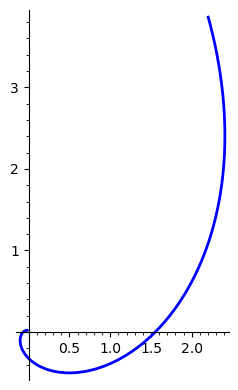
\includegraphics[scale=.6]{Images/ex4.2.png}
    \caption{New curve by curvature}
    \label{fig:ex4.2}
\end{figure}
\end{ex}

\section{Curvas Regulares no $\mathbb{R}^3$}\label{s5}


\bibliographystyle{sbc}
\bibliography{referencias}

\end{document}